% !TEX root = ../om_ts_02.tex

\begin{frame} % название фрагмента

\videotitle{Модель ETS(ANN)}

\end{frame}



\begin{frame}{Модель ETS(ANN): план}
  \begin{itemize}[<+->]
    \item Историческая справка о ETS. 
    \item ЕTS(ANN) как модель. 
    \item Формулы для прогнозов.
  \end{itemize}

\end{frame}

\begin{frame}{Историческая справка}

  \begin{itemize}[<+->]
    \item 1957-1960: Хольт и Винтерс придумали удачную формулу для прогнозирования.
  
    \item 2002: Роб Хиндман придумал статистические предпосылки для этой формулы.
    
    \item 2012: появился STAN — вероятностный язык программирования для байесовского оценивания.
    
    \item 2015: Славек Смыль описал обобщение ETS на STAN.
    
    \item 2017: PROPHET
    
    \item 2020: ORBIT
  \end{itemize}

\end{frame}

\begin{frame}{Терминология ETS}

  $y_t$ — наблюдаемый ряд;

  $\ell_t$ — тренд, очищенный ряд (\alert{единорог});

  $u_t$ — случайная ошибка.

  \pause
  \[
   y_t = \ell_{t-1} + u_t;
  \]
  \pause
  \[
  \ell_t = \ell_{t-1} + \alpha u_t, \text{ стартовое значение } \ell_0; 
  \]
  \pause
  \[
  u_t \sim \dN(0;\sigma^2) \text{ и независимы.}
  \]
  \pause

  Параметры: $\alpha$, $\sigma^2$, $\ell_0$.
\end{frame}

\begin{frame}{Смысл сокращения}

  ETS — \alert{Error, Trend, Seasonality} (ошибка, тренд, сезонность).

  \pause

  ANN — \alert{аддитивная} ошибка, \alert{нет} тренда, \alert{нет} сезонности.

\end{frame}


\begin{frame}{Не узнали?}

  ETS(ANN) — это обобщение \alert{случайного блуждания}.
  \pause

  \[
  \begin{cases}
   y_t = \ell_{t-1} + u_t; \\
  \ell_t = \ell_{t-1} + \alpha u_t, \text{ стартовое } \ell_0; \\
  u_t \sim \dN(0;\sigma^2) \text{ и независимы.} \\
  \end{cases}
  \]
  
  \pause
  Подставим $\alpha = 1$:
  \[
    y_t = \ell_t = \ell_{t-1} + u_t.  
  \]
  
\end{frame}


\begin{frame}
  \frametitle{Оценивание}

  Используется \alert{метод максимального правдоподобия}.

  \pause
  Основная идея: \alert{разложить} правдоподобие в сумму.

  \begin{multline*}
    \ln L(y \mid \theta) = \ln L(y_1 \mid \theta) + \ln L(y_2 \mid y_1, \theta) + \ldots + \\
     + \ln L(y_T \mid y_{T-1}, \ldots, y_1, \theta),
  \end{multline*}

  где $\theta = (\alpha, \ell_0, \sigma^2)$.

  \pause
  К сожалению, явных формул для оценок нет. 

\end{frame}

\begin{frame}
  \frametitle{Прогнозируем}

  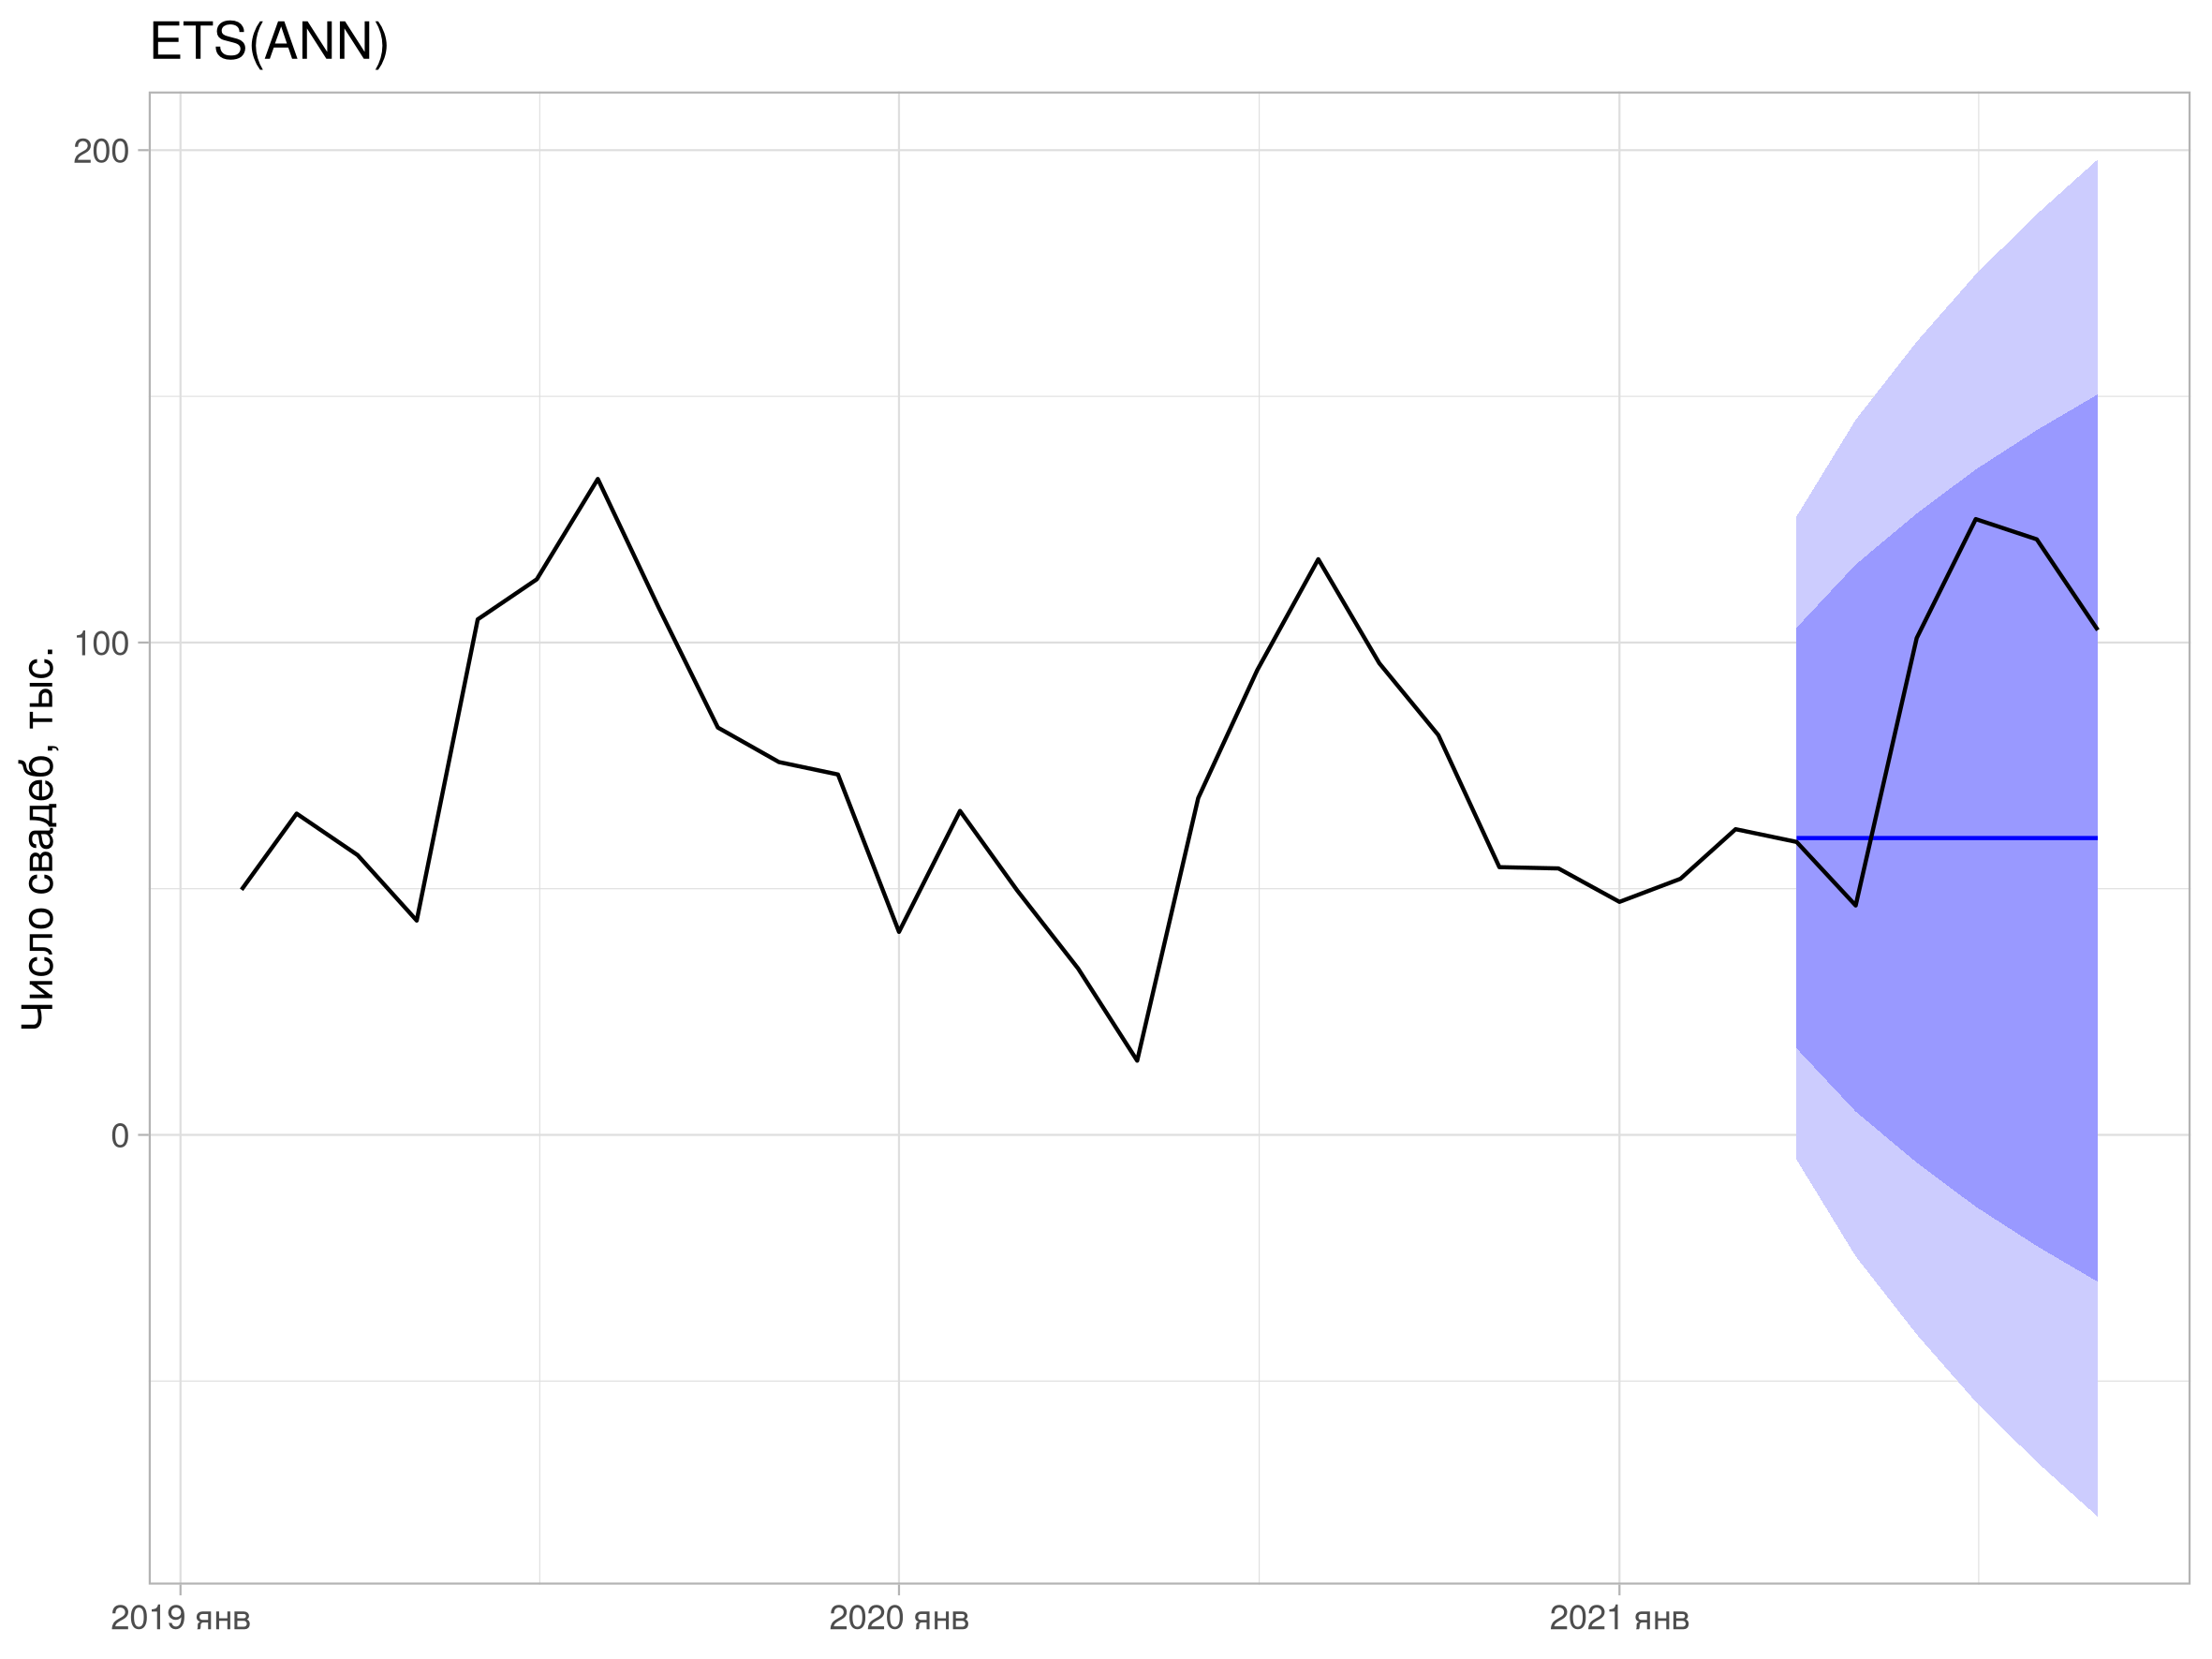
\includegraphics[width=\textwidth]{pictures/om_ts_02-025.png}
  

\end{frame}


\begin{frame}
  \frametitle{Прогноз на 1 шаг вперёд}

  К счастью, есть \alert{рекуррентные формулы} для прогнозов. 
  \pause

  \[
  \begin{cases}
   y_t = \ell_{t-1} + u_t; \\
  \ell_t = \ell_{t-1} + \alpha u_t, \text{ стартовое } \ell_0; \\
  u_t \sim \dN(0;\sigma^2) \text{ и независимы.}\\
  \end{cases}
  \]
  \pause
  \[
  y_{T+1} = \ell_T + u_{T+1}  
  \]
  \pause
  \[
  (y_{T+1} \mid \mathcal F_T) \sim \dN(\ell_T; \sigma^2)
  \]
  
\end{frame}


\begin{frame}
  \frametitle{Прогноз на 2 шага вперёд}

  \[
  \begin{cases}
   y_t = \ell_{t-1} + u_t;\\
  \ell_t = \ell_{t-1} + \alpha u_t, \text{ стартовое } \ell_0; \\
  u_t \sim \dN(0;\sigma^2) \text{ и независимы.}\\
  \end{cases}
  \]
  \pause
  \[
  y_{T+2} = \ell_{T+1} + u_{T+2} = \ell_T + \alpha u_{T+1} + u_{T+2} 
  \]
  \pause
  \[
  (y_{T+2} \mid \mathcal F_T) \sim \dN(\ell_T; \sigma^2(\alpha^2 + 1))
  \]
  
\end{frame}

\begin{frame}{Предиктивный интервал}

  Закон распределения
  \[
    (y_{T+2} \mid \mathcal F_T) \sim \dN(\ell_T; \sigma^2(\alpha^2 + 1))
  \]
  превращается в \pause \alert{предиктивный интервал}
  \[
  [\hat\ell_T - 1.96 \hat\sigma \sqrt{\hat\alpha^2 + 1}; \hat \ell_T + 1.96 \hat\sigma \sqrt{\hat\alpha^2 + 1}].
  \]
\end{frame}


\begin{frame}
  \frametitle{А что же открыли в 1950х?}

  \[
    \begin{cases}
     y_t = \ell_{t-1} + u_t;\\
    \ell_t = \ell_{t-1} + \alpha u_t, \text{ стартовое } \ell_0; \\
    \end{cases}
  \]  
  \pause 
  Перепишем второе уравнение:
  \[
  \ell_t = \ell_{t-1} + \alpha (y_t - \ell_{t-1}) = \alpha y_t + (1 - \alpha) \ell_{t-1}  
  \]

  \pause
  \alert{Простое экспоненциальное сглаживание}:

  \[
  \hat\ell_1 = y_1
  \]
  \pause
  \[
  \hat \ell_t = \alpha y_t + (1-\alpha) \hat \ell_{t-1}
  \]
  \pause
  \[
  \min_{\alpha} \sum (y_t - \hat \ell_t)^2;  
  \]
  
\end{frame}


\begin{frame}{ETS(ANN): итоги}

  \begin{itemize}[<+->]
    \item Формулы для \alert{экспоненциального сглаживания} были придуманы давно.
    \item Статистическая \alert{модель} ETS(ANN) появилась в 21 веке.
    \item Обобщение случайного блуждания. 
    \item \alert{Зёрнышко} огромного класса современных моделей.
  \end{itemize}
\end{frame}

